\subsubsection{Scope of interest}\label{sec:scope-of-interest}

The data models taken into consideration in this research must satisfy the requirements below:

\begin{enumerate}

    \item[R1)]\label{req:R1} They are currently used for data exchange between computer applications in the AEC/FM industry.

    \item[R2)] They were designed with the \emph{model-based} approach (see \ref{sec:glossary}) and they do not contain document data, for instance, text documents or drawings, which require interpretation by human.
    
    \item[R3)] Their data schemas are specified using one of the following formal data definition languages (DDLs): EXPRESS \cite{iso2004express}, XSD (XML Schema Definition) \cite{gao2009xsd, peterson2009xsd}, CSV (Comma-separated values) \cite{retter2016csv}, or SQL (Structured Query Language) \cite{iso2016sql, gulutzan1999sql}.
    
    \item[R4)] Their data can be stored either in one of the following serialisation formats: STEP Physical File \cite{iso2016stepfile}, XML, spreadsheet, CSV, and JSON (JavaScript Object Notation), or in relational data base management systems (RDBMS).     

    \item[R5)] Any class (or table) relationship, which is specified in the data schemas, either can be classified as an inheritance or an association, or can be ignored.
    
    % \item[R6] \emph{(optional)} Their atomic datatypes are based on or can be simplified to string, number, datetime, or boolean datatypes without semantic loss. 
    
    \item[R6)] \emph{(analysis needed)} Their atomic data types can be slightly modified, i.e. without semantic loss, in order to be primitive ones such as string, number, date, time, or boolean data types.
    
\end{enumerate}

These requirements are necessary to restrict the number of data models to those which have well-known properties and good potentials to be converted into OWL ontologies and RDF datasets.
On the one hand, most of data models widely used in the AEC/FM industry, especially the ones that are official or de-facto standards, comply with the requirements and belong to the scope of interest.
On the other hand, the examples below are not investigated in this research:
\begin{itemize}
    
    \item information models, which belong to other domains such as medicine or history, because they may use data structure patterns different to the typical ones in the AEC/FM product data models;
    
    \item native models, which are stored in the serialisation formats of specific application programs;
    
    % . However, most of them can be fully or partly converted by BIM tools into the IFC product model.
    
    \item data models, which contain sophisticated datatypes such as binary large objects (BLOBs), or arbitrary data types like \texttt{xsd:\-any\-Sim\-ple\-Ty\-pe} and \texttt{xsd:\-any\-Ty\-pe};
    
\end{itemize}


All three data levels of each data model, namely (1) data schema languages, (2) data schemas, and (3) datasets, are examined in term of conversion to Web of Data (see \autoref{fig:data-model-components}).
Definitions of schema languages, such as built-in data types, base data structures (e.g. enumerations, arrays, sets), or predefined constants, must be reflected in a separate OWL ontology.
Similarly, specific data schemas are mapped into a corresponding OWL ontologies.
Lastly, data instances from datasets are translated into RDF datasets.


\begin{figure}
    \centering    
    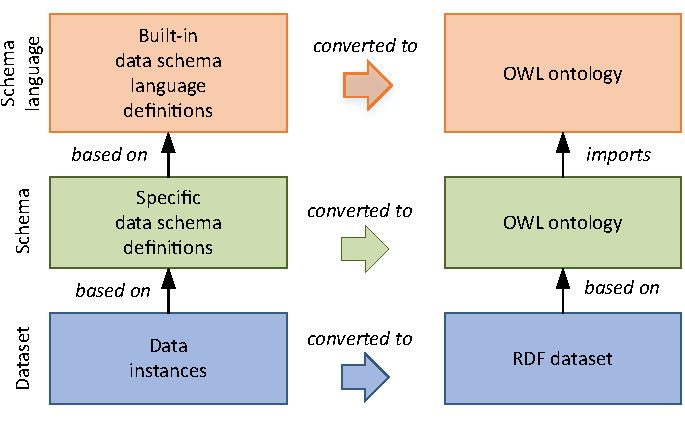
\includegraphics[width=\columnwidth]{images/data-model-components-2.pdf}
    \caption{Conversion of building data model to Web of Data}
    \label{fig:data-model-components}
\end{figure}


However, the research focuses only on the \emph{"pu\-re" sta\-tic mod\-el da\-ta} and ignores the rest part.
"Pure" model data consists of entities, explicit attributes and their values, which (a) represent a product model's state and (b) are needed for data exchange. 
In contrast, derived attributes, functions, procedures, and rules in EXPRESS language are never included in the datasets for data exchange.
Moreover, these elements contain executable statements, which cannot be represented in OWL 2 profiles.
Besides, worksheets, text styles, formulas, and procedures in spreadsheets are also \emph{out} of the question because they are unnecessary for data exchange between computer applications.
Furthermore, this is one of reasons of creating lightweight XML format COBieLite for COBie (Construction Operations Building Information Exchange) data (see \autoref{sec:data-model-classification}).



